% This poster was created using the baposter class,
% it was presented at the MoRePaS 2018 international
% conference, and can be viewed online here:
% https://doi.org/10.14293/P2199-8442.1.SOP-MATH.WTUXCF.v1

\documentclass[portrait,a0paper]{baposter}

%% Custom packages
\usepackage[utf8]{inputenc}
\usepackage[english]{babel}
\usepackage{lipsum}
\usepackage{float}
\usepackage{here}
\usepackage{fancyhdr}
\usepackage{mdwlist}
\usepackage{graphicx}
\usepackage{amssymb}
\usepackage{amsmath}
\usepackage{amsthm}
\usepackage{ifthen}
\usepackage{array}
\usepackage{tikz}
\usepackage{colortbl}
\usepackage{multicol}
\usepackage{xcolor}
\usepackage{comment}
\usepackage{tabularx}
\usetikzlibrary{shapes}
\usepackage{graphbox}
\usepackage{pgfplots}
\pgfplotsset{compat=1.9}
\usepackage[font=small,labelfont=bf,justification=centering]{caption}
\usepackage{natbib}
\usepackage{amsfonts}
\usepackage{amsmath}
\usepackage{stackengine}
\usepackage{siunitx}
\usepackage{booktabs}
\usepackage{enumitem}
\usepackage{tabularx}
\usepackage[none]{hyphenat}

%% Custom colors
% Define colors
\definecolor{ceatitlered}{HTML}{B71C1C}
\definecolor{ceatitle}{rgb}{0.4, 0.4, 0.4}
\definecolor{ceaframetitle}{rgb}{1, 1, 1}
\definecolor{ceagreen}{rgb}{0.58, 0.76, 0.11}
\definecolor{ceared}{rgb}{0.88, 0, 0.1}
\definecolor{ceablue}{rgb}{0.20, 0.47, 1}
\definecolor{ceablue2}{rgb}{0, 0, 1}
\colorlet{boxColor}{black!2}
%% Custom font
\usepackage[sfdefault]{FiraSans}
\makeatletter
\newcommand{\globalcolor}[1]{%
	\color{#1}\global\let\default@color\current@color
}
% random variables in sans serif font
\newcommand{\rvar}[1]{\mathsf{#1}} 
% random vectors in sans serif font
\newcommand{\rvec}[1]{\boldsymbol{\mathsf{#1}}} 
\makeatother
\AtBeginDocument{\globalcolor{black}}

%% Custom commands
% \newcommand{\captionfont}{\footnotesize}

%% Save space in lists. Use this after the opening of the list
\setlist[itemize]{leftmargin=10pt}
\setlist[enumerate]{leftmargin=10pt}
\newcommand{\compresslist}{%
\setlength{\itemsep}{1pt}%
\setlength{\parskip}{0pt}%
\setlength{\parsep}{0pt}%
}

\begin{document}
\begin{poster}%
%% Poster options
{
	grid=false,
	columns=3,
	colspacing=1em,
	bgColorOne=white,
	headerColorOne=white ,% mLightBrown!40,
	headerFontColor=gray!70!black, %mLightBrown!10!mDarkTeal,
	textborder=rectangle,
	borderColor=gray!70!black,
	eyecatcher=true,
	headerborder=none,
	headerheight=0.105\textheight,
	boxheaderheight=2.0em,
	headershape=smallrounded,
	headershade=plain,
	headerfont=\vphantom{\Huge X} \large\bfseries, %Sans Serif
	boxColorOne= red!3,% mLightBrown!20,
	background=plain,
	linewidth=1pt
}
	% Eye Catcher
{
	
 }
	% Title
{\bf  \begin{tabular}{c} \color{black!85} Principal component analysis \\ \color{black!85} and optimal weighted least-squares method\\ \color{black!85} for training tree tensor networks\end{tabular}}
	% Authors
{\hfill Cécile Haberstich \textsuperscript{1,2 \dag} \hfill Anthony Nouy \textsuperscript{1} \hfill Guillaume Perrin \textsuperscript{2} \hfill \vphantom{A}}
	% Logos
{
	\begin{tabular}{c}
		\includegraphics[height=1.4cm]{LogoLMJL} \includegraphics[height=1.4cm]{logocentrale}\\
		\hspace{-0.6cm}\includegraphics[height=1.4cm]{logoCEA}\\
	\end{tabular}
}

%% Boxes
\headerbox{}{name=contact,column=0,row=0,span=3,boxheaderheight=0em,boxColorOne=white,headerColorOne=white,textborder=none}{
	%	\textsuperscript{1} GeM, Centrale Nantes
	%	\par\smallskip	
	%	\textsuperscript{2} GeM, Université de Nantes
	%	\par\smallskip
	%	\textsuperscript{3} LMJL, Centrale Nantes
	%	\textsuperscript{1} Institut de Recherche en Génie Civil et Mécanique, Centrale Nantes
	%	\par\smallskip	
	%	\textsuperscript{2} Institut de Recherche en Génie Civil et Mécanique, Université de Nantes
	%	\par\smallskip
	%	\textsuperscript{3} Laboratoire de Mathématiques Jean Leray, Centrale Nantes
	%	\par\smallskip
	%	\textsuperscript{\dag} \textbf{\texttt{erwan.grelier@ec-nantes.fr}}
	\vspace{-.2cm}
	\begin{center}
		\begin{tabularx}{\textwidth}{XXX}
			\textsuperscript{1} LMJL (UMR CNRS 6629), Centrale Nantes&
			\textsuperscript{2} CEA/DAM/DIF, F-91297, Arpajon, France &
			\textsuperscript{\dag} \textbf{cecile.haberstich@ec-nantes.fr}
		\end{tabularx}
	\end{center}
	\vspace{-1.5cm}
}

\headerbox{References}{name=references,column=0,above=bottom,span=3,textborder=none}{
	\nocite{Nouy2017}
	\nocite{Cohen2016}
	\renewcommand{\section}[2]{}
	\bibliographystyle{abbrv}
	\bibliography{bibliography}
}

\headerbox{High-dimensional approximation}{name=UQ,column=0,below=contact,span=1,boxheaderheight=3em}{
We consider a pair of random variables \textcolor{gray!30!black}{$(X,Y)$} such that \textcolor{red!60!black}{$Y = u(X)$}, where $X = (X_1,...,X_d)$ is a random vector and $u : \mathcal{X} \to \mathbb{R}$ is a function.\\
In the context of \textcolor{red!60!black}{Uncertainty Quantification}, $Y$ is the output of a numerical code and $X$ are the input parameters.\\
When $u$ is costly to evaluate, we replace $u$ by an \textcolor{red!60!black}{approximation $u^*$}.

\vspace{0.3cm}
\textcolor{gray!50!black}{\textbf{Objectives:}}
\begin{itemize}\compresslist
	\vspace{-0.3cm}
	\item Construct an approximation $u^*$ using only a \textcolor{gray!30!black}{few evaluations of $u$}
	\item Exploit \textcolor{red!60!black}{low-rank structures}
	\item Propose a sample-based algorithm with \textcolor{red!60!black}{guaranteed stability}
\end{itemize} 
}

\headerbox{\begin{tabular}{c}
	Higher-order principal component analysis\\for tree-based formats
	\end{tabular} }{name=algo,column=1,span=1,below=contact,boxheaderheight=3em}{
	The \textcolor{red!60!black}{best approximation of $u$ by a function with $\alpha$-rank $r_\alpha$} is the truncated singular value decomposition:
	\vspace{-0.3cm}
	\begin{equation}
	\nonumber
	u_{r_{\alpha}}(x_{\alpha}, x_{\alpha^c})  = \sum_{k=1}^{\textcolor{red!60!black}{r_{\alpha}}} \sigma_k \textcolor{red!60!black}{v_k^{\alpha}}(x_{\alpha})v_k^{\alpha^c}(x_{\alpha^c})
	\end{equation}
	$\textcolor{red!60!black}{v_1^{\alpha}},..., \textcolor{red!60!black}{v_{r_{\alpha}}^{\alpha}}$ are the \textcolor{red!60!black}{$r_{\alpha}$ $\alpha$-principal components of $u$} and $\textcolor{red!60!black}{\text{span}\{v_1^{\alpha},...,v_{r_{\alpha}}^{\alpha}\} = U_{\alpha}}$ is the \textcolor{red!60!black}{$\alpha$-principal subspace} of $u$.
	
	\vspace{0.3cm}
	\textcolor{gray!50!black}{\textbf{Extension to tree-based formats:}}\\
	From the leaves of the tree to the root, determine the subspaces $U_{\alpha}$ of principal components of $u_{\alpha} = \mathcal{P}_{V_{\alpha}}u$ for all $\alpha$, with $\mathcal{P}_{V_\alpha}$ the orthogonal projection onto $U_{\alpha} \otimes L^2_{\mu_{\alpha}}$:
	\vspace{-0.8 cm}
		\begin{center}
		$$
		\begin{array}{cc} 
		\hspace{-0.2cm}\text{if $S(\alpha) = \emptyset$, $V_{\textcolor{red!70}{\alpha}}$ is a given} & \text{if $S(\alpha)\neq \emptyset$} \\
		\text{approximation space} & V_{\alpha} = \otimes_{\textcolor{red!40}{\beta} \in S(\textcolor{red!70}{\alpha})} U_{\textcolor{red!40}{\beta}}\\
			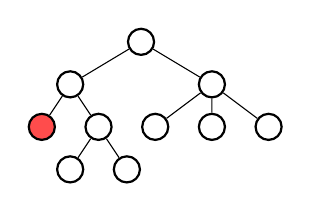
\begin{tikzpicture}[scale=.9,yscale=.4]
			\tikzstyle{level 1}=[sibling distance=20mm]
			\tikzstyle{level 2}=[sibling distance=8mm]
			\tikzstyle{root}=[circle,minimum size=.25cm, draw,thick,fill=white]
			\tikzstyle{interior}=[circle,draw,minimum size=.25cm,solid,thick,fill=gray!20]
			\tikzstyle{leaves}=[circle,draw,minimum size=.25cm,solid,thick,fill=gray!20]
			\tikzstyle{active}=[circle,draw,minimum size=.25cm,solid,thick,fill=red!70]
			\tikzstyle{inactive}=[circle,draw,minimum size=.25cm,solid,thick,fill=white]
			
			\node [root,fill=white] {}
			child {node [inactive]  {}
				child { node [active] {}} 
				child { node [inactive] {}
					child { node [inactive] {}} 
					child { node [inactive] {}}   }      }
			child {node [inactive] {}
				child { node [inactive] {}} 
				child { node [inactive] {}}   
				child { node [inactive] {}}    }
			;
			\end{tikzpicture}
			&
			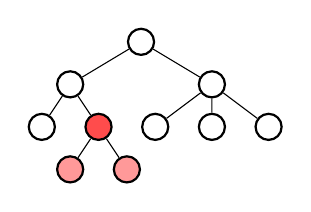
\begin{tikzpicture}[scale=.9,yscale=.4]
			\tikzstyle{level 1}=[sibling distance=20mm]
			\tikzstyle{level 2}=[sibling distance=8mm]
			\tikzstyle{root}=[circle,minimum size=.25cm,draw,thick,fill=white]
			\tikzstyle{sons}=[circle,minimum size=.25cm,draw,solid,thick,fill=red!40]
			\tikzstyle{leaves}=[circle,minimum size=.25cm,draw,solid,thick,fill=gray!20]
			\tikzstyle{active}=[circle,minimum size=.25cm,draw,solid,thick,fill=red!70]
			\tikzstyle{inactive}=[circle,minimum size=.25cm,draw,solid,thick,fill=white]
			
			\node [root,fill=white] {}
			child {node [inactive]  {}
				child { node [inactive] {}} 
				child { node [active] {}
					child { node [sons] {}} 
					child { node [sons] {}}   }      }
			child {node [inactive] {}
				child { node [inactive] {}} 
				child { node [inactive] {}}   
				child { node [inactive] {}}    }
			;
			\end{tikzpicture}
			
		\end{array}
		$$
		\end{center}
		Finally project u onto the tensor space $ \otimes_{\textcolor{red!70}{\alpha} \in S(D)} U_{\textcolor{red!70}{\alpha}}$, to obtain the approximation\\
		$u^* =  \prod_{\textcolor{red!70}{\alpha} \in S(D)} \mathcal{P}_{U_{\textcolor{red!70}{\alpha}}} u$
		\vspace{-0.6cm}
		$$
		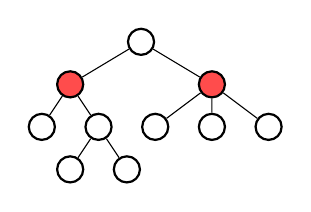
\begin{tikzpicture}[scale=.9,yscale=.4]
		\tikzstyle{level 1}=[sibling distance=20mm]
		\tikzstyle{level 2}=[sibling distance=8mm]
		\tikzstyle{root}=[circle,minimum size=.25cm,draw,thick,fill=white]
		\tikzstyle{sons}=[circle,minimum size=.25cm,draw,solid,thick,fill=blue]
		\tikzstyle{leaves}=[circle,minimum size=.25cm,draw,solid,thick,fill=gray!20]
		\tikzstyle{active}=[circle,minimum size=.25cm,draw,solid,thick,fill=red!70]
		\tikzstyle{inactive}=[circle,minimum size=.25cm,draw,solid,thick,fill=white]
		
		\node [root,fill=white] {}
		child {node [active]  {}
			child { node [inactive] {}} 
			child { node [inactive] {}
				child { node [inactive] {}} 
				child { node [inactive] {}}   }      }
		child {node [active] {}
			child { node [inactive] {}} 
			child { node [inactive] {}}   
			child { node [inactive] {}}    }
		;
		\end{tikzpicture}
		$$
\textcolor{gray!50!black}{\textbf{Control of the error}}:
	\begin{itemize}
		\vspace{-0.3cm}
		\item algorithm with \textcolor{red!60!black}{prescribed rank}:
		\vspace{-0.3cm}
		\begin{equation}
		\nonumber
		\hspace{-0.3cm} \Vert u-u^* \Vert ^2 \leq \# T \min_{v \in T_r^T} \Vert v - u \Vert^2 + \hspace{-0.2cm} \sum_{\alpha \in \mathcal{L}(T)} \Vert u-\mathcal{P}_{V_{\alpha}}u \Vert ^2
		\end{equation}
		\vspace{-0.8cm}
		\item algorithm with \textcolor{red!60!black}{prescribed tolerance}:
		
		\vspace{-0.1cm}
		if $\Vert u - \mathcal{P}_{V_{\alpha}}u \Vert \le \epsilon/\sqrt{d} \Vert u \Vert$
		
		\vspace{-0.1cm}
		and if $r_{\alpha}$ is chosen such that:
		
		\vspace{-0.1cm}
		$ \Vert u_{\alpha} - \mathcal{P}_{U_{\alpha}} u_{\alpha}\Vert \le \epsilon/\sqrt{\#T} \Vert u_{\alpha} \Vert$
		
		\vspace{-0.1cm}
		then $\Vert u- u^* \Vert \le \epsilon \Vert u \Vert$
	\end{itemize}
\vspace{0.01cm}
}

\headerbox{Statistical estimation of principal components $U_{\alpha}$}{name=stat,column=0,below=algo, span=2}{

\begin{multicols}{2}
In practice we determine $U_{\alpha}$ by solving: 
\vspace{-0.3cm}
\begin{equation}
\nonumber
\hspace{-0.15cm} \min_{\dim(U_{\alpha})=r_{\alpha}} \frac{1}{n_{\alpha}} \sum_{k=1}^{n_{\alpha}} \left\Vert  u_{\alpha}(\cdot,x_{\alpha^c}^k) - P_{U_{\alpha}}u_{\alpha}(\cdot,x_{\alpha^c}^k) \right \Vert^2_{L^2_{\mu_{\alpha}}}
\vspace{0.4cm}
\end{equation}
$(x_{\alpha^c}^k)_{k=1}^{n_{\alpha}}$ are i.i.d. samples of the group of variables $x_{\alpha^c}$\\ $P_{U_{\alpha}} \text{is the orthogonal projection onto } U_{\alpha}.$
\end{multicols}
}

\headerbox{Tree-Based Tensor formats}{name=TBT,column=0, below=UQ,above=stat}{
	$u$ is in $L^2_{\mu}$, with $\mu$ a product probability measure on $\mathcal{X}$.\\ $L^2_{\mu}$ is identified with $L^2_{\mu_1} \otimes ... \otimes L^2_{\mu_d}$.\\
	For $\alpha \subset D = \{1,...,d\}$, $u$ is identified with a bivariate function in $L^2_{\mu_{\alpha}} \otimes L^2_{\mu_{\alpha^c}}$.\\
	A function \textcolor{red!60!black}{$u$ with $\alpha$-rank $r_{\alpha}$:}
	\begin{equation}
	\nonumber
	u(x_{1},...,x_{d}) = \sum_{i=1}^{r_{\alpha}} v^{\alpha}_{i}(x_{\alpha})v^{\alpha^c}_{i}(x_{\alpha^c})
	\end{equation}
	
	\vspace{-0.3cm}
	If a function $u$ has the above representation for all $\alpha \in T$ where $T \subset 2^{\{1,...d\}}$, and $T$ is a dimension partition tree, \textcolor{red!60!black}{$u$ has a representation in tree-based tensor format $\mathcal{T}_r^T$}.
	$$
	\begin{array}{c} \footnotesize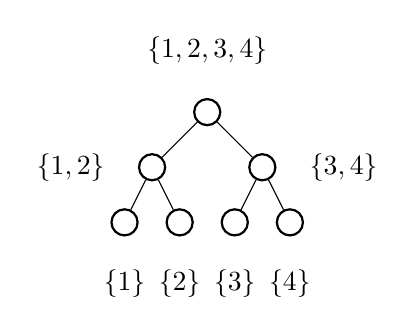
\begin{tikzpicture}[scale=0.7,level distance = 10mm,baseline=(current bounding box.south),label distance=3mm]
	\tikzstyle{level 1}=[sibling distance=20mm]
	\tikzstyle{level 2}=[sibling distance=10mm]
	\tikzstyle{root}=[circle,minimum size=.25cm,draw,thick,fill=white]
	\tikzstyle{interior}=[circle,minimum size=.25cm,draw,solid,thick]
	\tikzstyle{leaves}=[circle,minimum size=.25cm,draw,solid,thick]
	\tikzstyle{active}=[circle,minimum size=.25cm,draw,solid,thick]
	
	\node [root,label=above:{$\{1,2,3,4\}$},]  {}
	child {node [interior,label=left:{$\{1,2\}$}]  {} 
		child { node [leaves,label=below:{$\{1\}$}] {}} 
		child { node [interior,label= below:{$\{2\}$}] {}
		}  }
		child {node [interior,label= right:{$\{3,4\}$}]  {}
			child { node [leaves,label=below:{$\{3\}$}] {}}
			child { node [leaves,label=below:{$\{4\}$}] {}}  }
		;
		\end{tikzpicture}\\ \footnotesize{\text{A dimension partition tree T over $D = \{1,2,3,4\}$}}
		\end{array}
		$$
	}


\headerbox{Optimal Weighted Least-Squares}{name=OWLS,column=2,below=contact,above=stat}{
PCA involves projections $P_Vu$ with\\
$V = V_{\alpha}$ or $V = U_{\alpha}$ subspaces of $L^2_{\mu_{\alpha}}$.\\
For a function $f \in L^2_{\rho}$, replace the ideal \textcolor{red!60!black}{orthogonal projection:}
	\vspace{-0.3cm}
\begin{equation}
\nonumber
P_{V}f= \arg\min_{v \in W} \|v-f\|_{L^2_{\rho}}
\vspace{-0.3cm}
\end{equation}
 by a \textcolor{red!60!black}{weighted least-squares projection}:
	\vspace{-0.3cm}
	\begin{equation}
	\nonumber
	P^w_{V}f = \arg\min_{v \in V} \frac{1}{n} \sum_{i=1}^{n}w^i\lvert v(z^i) - f(z^i) \lvert ^2
	\vspace{-0.3cm} 
	\end{equation}
with $(z^i)_{i=1}^n$ i.i.d samples from the measure $d\rho_w$.\\
$\Vert 	P^w_{V}f-f \Vert_{L^2_{\rho}}$ should be close to the error of best approximation and $n$ as close as possible to $m$, the dimension of $V$.

\vspace{0.2cm}
\textcolor{gray!50!black}{\textbf{Optimal choice \cite{Cohen2016}}}:
	\begin{enumerate}\compresslist
			\vspace{-0.3cm}
		\item Sample $(z^i)_{i=1}^n$ from $d\rho_w = w^{-1}d\rho$ with $w^{-1}(z)
 = \frac{1}{m}\sum_{i=1}^{m} \varphi_i(z)^2$ where $(\varphi_i)_{i=1}^m$ is an orthonormal basis of $V$
 		\item Choose weigths $(w^i)_{i=1}^n = (w(z^i))_{i=1}^n$ %to ensure $\lim\limits_{n \rightarrow \infty}\|v\|_n = \|v\|$
	\end{enumerate}
	The condition \textcolor{red!60!black}{$n \ge c(r) m \log(m)$} ensures the stability property:
		\vspace{-0.3cm}
	\textcolor{red!60!black}{
	\begin{equation}
	\nonumber
	Pr\{\Vert G - I \Vert \ge \frac{1}{2}\} \le m^{-r}
	\vspace{-0.3cm}
	\end{equation}}

	\vspace{-0.3cm}
	with $G$ the empirical grammian matrix of basis $(\varphi_i)_{i=1}^m$
	\begin{center}
	\vspace{-0.3cm}
	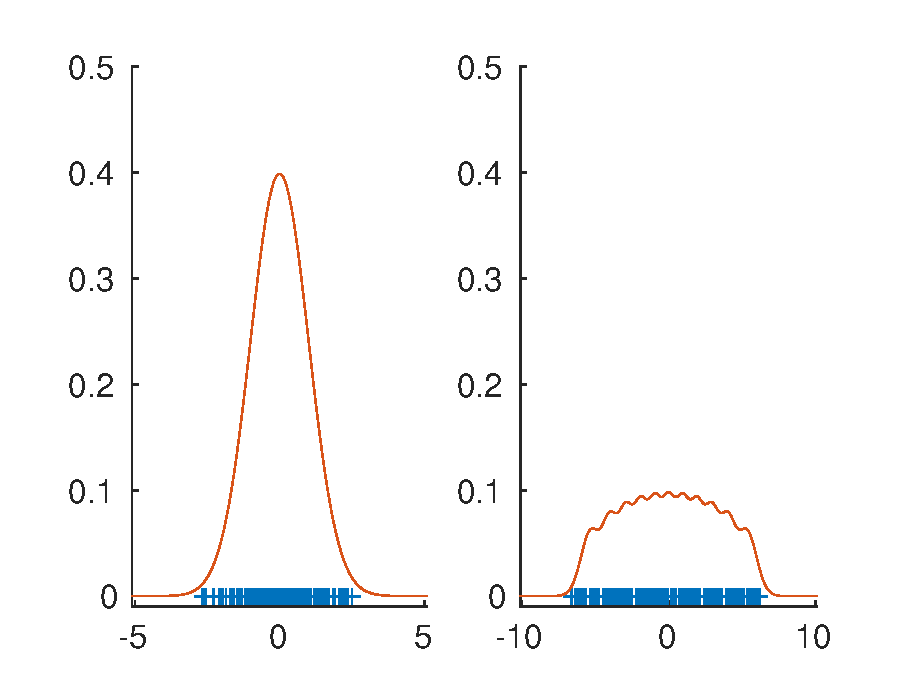
\includegraphics[scale=0.40]{OWLS}\\
	\footnotesize{Left: Pdf and samples of the gaussian measure $\rho$,\\ Right: Pdf and samples of the weighted measure $\rho_w$ with $m=11$}
	\end{center}
	\vspace{-0.3cm}
	The sampling according to optimal measures exploits the tensor product structure of the functions involved.
}

\headerbox{Numerical experiments $f(x) = \sin(\sum_{i=1}^{10} x_i)$ }{name=scaling,column=0,span=2,below=stat, above=references}{%$
We consider $\mathcal{X} = \mathbb{R}^d$, with the standard Gaussian measure, and a fixed $\alpha$-rank equal to 2.\\
\vspace{-0.2cm}
$$
\begin{array}{c|ccc|ccc}
\hspace{-0.3cm}\text{polynomial degree of} & \multicolumn{3}{c}{\text{Approximation error in $\log_{10}$}} & \multicolumn{3}{c}{\text{Number of samples}}\\
\hspace{-0.3cm} \text{the approximation basis} & \text{WLS} & \text{SLS} & \text{Interpolation} & \text{WLS} & \text{SLS} & \text{Interpolation} \\ \hline
5 & \hspace{-0.3cm}[-1.1, -0.9] & [-1, -0.1] & [-0.6, -0.4] & 1292 & 1292 & 188\\
10 & \hspace{-0.3cm}[-3.6, -3.5] & [-3.4, -2.3] & [-4.3, -3.9] & 2212 & 2212 & 288\\
20 & \hspace{-0.3cm}[-9.8, -9.5] & [-9.7, -7.5] & [-13.2, -10.8] & 4232 & 4232 & 488\\
25 & \hspace{-0.1cm}[-13.3, -12.9] & [-8.8, -4.1] & [-13.1, -8.4] & 5292 & 5292 & 588\\
40 & \hspace{-0.2cm}[-14.5, -14] & [-7.4, -2.5] & \text{error} & 8652 & 8652 &  \text{error}\\
\end{array}
$$
}

\headerbox{Conclusions}{name=conclusions,column=2,span=1,below=OWLS,above=references}{%
The optimal-weighted projection in the higher-order PCA algorithm \textcolor{red!60!black}{increases the stability} compared to a standard least-squares projection or interpolation. This stability is guaranteed with conditions on the number of samples.

\vspace{0.2cm}
\textcolor{gray!50!black}{\textbf{Ongoing works}}: 
\vspace{-0.3cm}
	\begin{itemize}\compresslist
		\item For a fixed rank, provide conditions on the number of samples $n_{\alpha}$ that garantee a quasi-optimality result in expectation or probability for the empirical PCA
		\item Provide fully \textcolor{red!60!black}{adaptive algorithms} (in samples, ranks) that achieve (in expectation or high probability) a prescribed precision
		\item Exploit \textcolor{red!60!black}{sparsity} of tensors
	\end{itemize}
}




\end{poster}
\end{document}